% Relatorio do T2 (mestre/escravo com MPI). Compilar: cd relatorio && pdflatex relatorio.tex && pdflatex relatorio.tex
% As tabelas (tab_*.tex) e figuras (fig_*.pdf) sao geradas por: python3 scripts/analyze.py
\documentclass[10pt,twocolumn,a4paper]{article}
\usepackage[utf8]{inputenc}
\usepackage[T1]{fontenc}
\usepackage{lmodern}
\usepackage[a4paper,margin=1.5cm,columnsep=0.6cm]{geometry}
\usepackage{booktabs}
\usepackage{graphicx}
\usepackage{caption}
\usepackage{amsmath}
\usepackage{microtype}
\usepackage[hidelinks]{hyperref}
\usepackage{titlesec}
\titlespacing*{\section}{0pt}{4pt}{1pt}
\titleformat{\section}{\normalsize\bfseries}{\thesection.}{0.4em}{}
\captionsetup{font=small,labelfont=bf,skip=2pt}
\setlength{\parskip}{0pt}
\setlength{\parindent}{0.8em}
\setlength{\textfloatsep}{6pt}
\setlength{\dbltextfloatsep}{6pt}
\setlength{\dblfloatsep}{6pt}
\setlength{\abovecaptionskip}{3pt}
\setlength{\belowcaptionskip}{0pt}
\setlength{\tabcolsep}{3pt}
\renewcommand{\topfraction}{0.95}\renewcommand{\dbltopfraction}{0.95}
\renewcommand{\textfraction}{0.03}\renewcommand{\floatpagefraction}{0.9}\renewcommand{\dblfloatpagefraction}{0.9}
\setcounter{topnumber}{4}\setcounter{dbltopnumber}{4}\setcounter{totalnumber}{6}
\newcommand{\code}[1]{\texttt{#1}}
\newcommand{\lref}[2]{\code{#1}:#2}
\pagestyle{empty}
\AtBeginDocument{\renewcommand{\figurename}{Figura}\renewcommand{\tablename}{Tabela}}

\begin{document}
\twocolumn[{%
\begin{center}
{\large\bfseries T2 -- Conjunto de Julia com MPI no modelo mestre/escravo}\\[2pt]
Francisco Freitas e Pedro Haggstram \quad$\cdot$\quad
Repositório: \url{https://github.com/fcmfreitas/c_mpi}
\end{center}
\vspace{2pt}
}]

% Floats largos: o LaTeX os coloca no topo da pagina seguinte a onde aparecem.
\begin{table*}[t]
\centering\scriptsize
\IfFileExists{tab_gran.tex}{\begin{tabular}{lrrrrrrrrr}
\toprule
linhas/tarefa & tarefas & mediana (s) & min (s) & max (s) & tarefa (ms) & ida e volta intra ($\mu$s) & inter ($\mu$s) & util. & cauda (s) \\
\midrule
1 & 2160 & 1,66 & 1,66 & 1,67 & 23,6 & 12 & 248 & 99\% & 0,00 \\
2 & 1080 & 1,66 & 1,66 & 1,66 & 47,2 & 14 & 382 & 99\% & 0,00 \\
4 & 540 & 1,66 & 1,66 & 1,66 & 94,3 & 19 & 653 & 99\% & 0,01 \\
8 & 270 & 1,67 & 1,67 & 1,67 & 188,7 & 30 & 808 & 98\% & 0,03 \\
16 & 135 & 1,81 & 1,79 & 1,82 & 376,0 & 53 & 871 & 90\% & 0,27 \\
32 & 68 & 2,27 & 2,25 & 2,31 & 739,0 & 96 & 1434 & 71\% & 1,02 \\
64 & 34 & 2,58 & 2,55 & 2,62 & 1472,0 & 177 & 2596 & 63\% & 2,33 \\
128 & 17 & 4,71 & 4,44 & 4,73 & 2938,5 & 342 & 4913 & 34\% & 4,70 \\
256 & 9 & 8,97 & 7,89 & 9,01 & 5395,7 & 985 & 9600 & 18\% & 8,97 \\
512 & 5 & 14,56 & 13,47 & 15,71 & 9362,7 & 3020 & 18905 & 10\% & 14,56 \\
\bottomrule
\end{tabular}
}{(tab\_gran.tex)}
\caption{Granularidade com $P=32$ (31 escravos), 10 execuções por linha: tempo total; tempo médio de
uma tarefa (ocupado/tarefas); ida e volta das mensagens de uma tarefa, sem cálculo, com escravos do nó
do mestre (intra) e do outro (inter); util.\ = fração do tempo em que os escravos calculam; cauda = do
primeiro escravo liberado ao fim.}
\label{tab:gran}
\end{table*}

\section{Modelagem}
O problema é o do T1: cada pixel $z_0$ itera $z \leftarrow z^2 + c$ com $c=-0{,}123+0{,}745i$
(interior do conjunto de Mandelbrot, então os pixels do interior custam \code{max\_iter}
iterações), e cada pixel independe dos demais. \textbf{Tarefa:} bloco de \code{chunk} linhas
consecutivas, lido da linha de comando (\lref{julia\_common.c}{50}). \textbf{Saco:} o mestre
(rank 0) guarda só o índice da próxima linha livre, \code{next\_row}; há $\lceil
\text{linhas}/\code{chunk}\rceil$ tarefas, a última pode ser menor, e qualquer número de linhas e
de processos ($P\ge2$) funciona (\lref{julia\_mpi.c}{47--57}). \textbf{Tags}
(\lref{julia\_mpi.c}{21}): \code{TAG\_REQUEST} (escravo$\to$mestre, vazia: primeiro pedido, l.~89);
\code{TAG\_PIXELS} (escravo$\to$mestre, \{primeira linha, pixels\}: resultado que vale como pedido
da próxima tarefa, l.~103); \code{TAG\_WORK} (mestre$\to$escravo, \{primeira linha, linhas\},
l.~54); \code{TAG\_DONE} (mestre$\to$escravo, vazia, l.~49). O mestre recebe com
\code{MPI\_ANY\_SOURCE}/\code{MPI\_ANY\_TAG} (l.~71), atende por ordem de chegada e não calcula.
\textbf{Ordem:} o resultado traz sua primeira linha em \code{block[0]} e é copiado direto para essa
posição da imagem (l.~77), qualquer que seja a ordem de chegada. \textbf{Término:} com o saco vazio
cada pedido é respondido com \code{TAG\_DONE}; o escravo sai do laço ao vê-la (l.~94) e o mestre
encerra quando liberou os $P-1$ escravos (l.~79--83).

\section{Ambiente e metodologia}
Tudo rodou no cluster Atlântica do LAD, sempre nos nós \code{atlantica07} e \code{atlantica08}
com \code{--exclusive}, por jobs \code{sbatch} (\code{scripts/t2\_*.sbatch}; saídas brutas e
\code{lscpu} em \code{results/}). \textbf{Cada nó tem 2 Xeon E5520 de 4 núcleos com HT: 8 núcleos
físicos e 16 threads} (não 16/32 como supõe o enunciado), 16\,GB e Gigabit Ethernet; por isso
$P=2,4,8$ ficam em um nó com 1 processo por núcleo físico (\code{--cpu-bind=cores}), $P=16$ em 2
nós $\times$ 8 núcleos, $P=32$ em 2 nós $\times$ 16 threads (o ponto ``HT'') e $P=64$ com 2
processos por thread (\code{--overcommit}, \code{OMPI\_MCA\_mpi\_yield\_when\_idle=1}). Os ranks
preenchem os nós em bloco; o mestre (rank 0) e a sequencial ficam sempre no \code{atlantica07}.
\code{gcc 9.4.0} via \code{mpicc} (OpenMPI 4.1.1), \code{-O3 -march=native}, compilado no nó de
cômputo, para as duas versões. \textbf{Região medida:} \code{MPI\_Wtime} no mestre após um
\code{MPI\_Barrier}, do início da distribuição à chegada do último resultado
(\lref{julia\_mpi.c}{202--208}); na sequencial, \code{clock\_gettime} em volta do laço de linhas
(\lref{julia\_seq.c}{52--55}); alocação, checksum e saída ficam fora. \textbf{Entrada de
referência:} $3840\times2160$ (2160 linhas), \code{max\_iter}~$=6000$, calibrada para
$T_1\in[30,60]$\,s. \textbf{Fraca:} a região do plano é fixa, então \code{--height}~$=2160P$ só
adensa a amostragem vertical: as tarefas crescem com $P$ e o custo médio de uma linha não muda (as
iterações totais confirmam, Tabela~\ref{tab:escala}). Cada configuração rodou 10 vezes em
processos independentes (mediana, mínimo e máximo nas tabelas) e \textbf{toda execução imprimiu
iterações e checksum FNV-1a da imagem, iguais aos da sequencial com a mesma entrada}
(\code{results/resumo.md}).

\section{Granularidade e balanceamento}
\begin{figure*}[t]
\centering
\IfFileExists{fig_curvas.pdf}{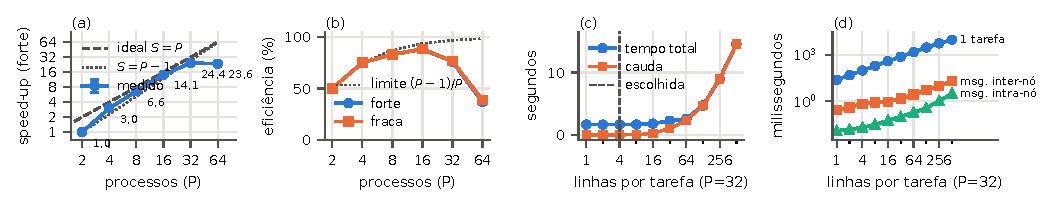
\includegraphics[width=\textwidth]{fig_curvas.pdf}}{(fig\_curvas.pdf)}
\caption{(a) Speed-up da forte com a reta ideal e $S=P-1$ (mestre sem calcular); (b) eficiência da
forte e da fraca com o limite $(P-1)/P$; (c) $P=32$: tempo total (mediana, faixa min--max) e cauda por
granularidade; (d) custo de uma tarefa contra a ida e volta das suas mensagens, intra e inter-nó.}
\label{fig:curvas}
\end{figure*}
\begin{figure*}[t]
\centering
\IfFileExists{fig_balance.pdf}{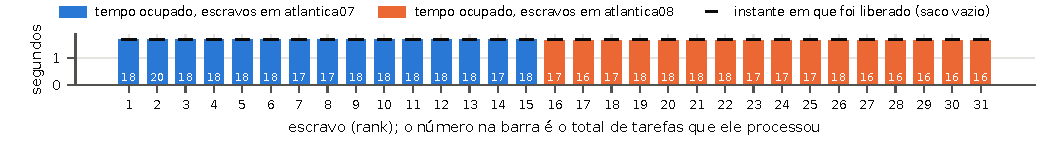
\includegraphics[width=\textwidth]{fig_balance.pdf}}{(fig\_balance.pdf)}
\caption{Balanceamento com $P=32$ e 4 linhas por tarefa (mediana de 10 execuções): tempo ocupado e
tarefas por escravo, cor por nó, e instante em que cada um recebeu \code{TAG\_DONE}.}
\label{fig:balance}
\end{figure*}
A Tabela~\ref{tab:gran} e a Figura~\ref{fig:curvas}(c,d) comparam, com $P=32$, a granularidade
escolhida (\textbf{4 linhas por tarefa}, 540 tarefas) com granularidades bem menores (1 linha,
2160 tarefas) e bem maiores (até 512 linhas, 5 tarefas). \textbf{Computação vs.\ comunicação:}
uma tarefa de 4 linhas custa 94\,ms de cálculo; a ida e volta das suas mensagens (61\,KB de
pixels e 8 bytes de tarefa, sem cálculo) custa 19\,$\mu$s no mesmo nó e 653\,$\mu$s entre nós:
razões de 5000 e 140. A rede Gigabit domina a comunicação inter-nó (0,25\,ms de latência mais
0,13\,ms por linha de 15\,KB) e é 30 vezes mais lenta que a memória compartilhada. Como cada
escravo só espera uma ida e volta por tarefa (no máximo 0,7\% do seu tempo) e o mestre gasta
dezenas de microssegundos por mensagem, \textbf{1, 2, 4 e 8 linhas dão o mesmo tempo
(1,66--1,67\,s)}; 4 linhas foi escolhida por cortar as mensagens de 2160 para 540 sem custo
medido. \textbf{Granularidades maiores} perdem por desbalanceamento no fim do saco, não por
comunicação: as linhas têm custos muito diferentes (as que cruzam o interior do conjunto custam
\code{max\_iter} por pixel, as da borda quase nada), então com poucas tarefas a última tarefa cara
de cada escravo acaba em instantes distintos. Com 16 linhas (135 tarefas, 4 por escravo) a cauda
já é de 0,27\,s; com 32 linhas (68 tarefas), 1,0\,s dos 2,27\,s totais, e a utilização cai a
71\%; com 128 linhas (17 tarefas) 14 escravos nunca recebem trabalho e o tempo é o da tarefa mais
cara (4,7\,s). \textbf{Balanceamento com 4 linhas} (Figura~\ref{fig:balance}): os 31 escravos
ficam ocupados de 1,63 a 1,65\,s (99\% do tempo) e são liberados no mesmo instante ($\pm2$\,ms),
com 16 a 20 tarefas cada; a variação vem do custo desigual das tarefas e da espera 0,65\,ms maior
dos escravos do segundo nó, que pegam uma ou duas a menos.

\section{Resultados}
\begin{table*}[t]
\centering\scriptsize
\IfFileExists{tab_escala.tex}{\begin{tabular}{r rrr rr rr | rrr rr r}
\toprule
& \multicolumn{7}{c|}{forte (entrada de referência)} & \multicolumn{6}{c}{fraca (\code{height} $=2160P$)} \\
$P$ & $T_P$ (s) & min & max & $S$ & $E$ & CPU/$T_1$ & cauda (s) & $T_P$ (s) & min & max & $E_\text{fraca}$ & iter./iter.$_1$ & equiv. \\
\midrule
2 & 40,34 & 40,33 & 40,34 & 1,0 & 50\% & 1,00 & 0,00 & 80,7 & 80,7 & 80,7 & 50\% & 2,00 & ok \\
4 & 13,45 & 13,45 & 13,58 & 3,0 & 75\% & 1,00 & 0,00 & 53,8 & 53,8 & 54,3 & 75\% & 4,00 & ok \\
8 & 6,08 & 6,08 & 6,08 & 6,6 & 83\% & 1,05 & 0,00 & 48,6 & 48,6 & 48,7 & 83\% & 8,00 & ok \\
16 & 2,87 & 2,86 & 2,87 & 14,1 & 88\% & 1,05 & 0,00 & 45,6 & 45,6 & 45,7 & 89\% & 16,00 & ok \\
32 & 1,66 & 1,66 & 1,66 & 24,4 & 76\% & 1,26 & 0,01 & 52,9 & 52,8 & 52,9 & 76\% & 32,00 & ok \\
64 & 1,71 & 1,68 & 1,76 & 23,6 & 37\% & 2,40 & 0,08 & 104,6 & 104,5 & 104,8 & 39\% & 64,00 & ok \\
64 (polling) & 1,76 & 1,72 & 1,86 & 22,9 & 36\% & 2,49 & 0,08 & -- & -- & -- & -- & -- & -- \\
\bottomrule
\end{tabular}
}{(tab\_escala.tex)}
\caption{Forte (entrada de referência; $T_1=40{,}41$\,s, mín.\ 40,35, máx.\ 40,42) e fraca
(\code{height}~$=2160P$), 10 execuções por linha: $T_P$ (mediana, mín., máx.), $S=T_1/T_P$, $E=S/P$,
$E_\text{fraca}=T_1/T_P$; CPU/$T_1$ = tempo ocupado total dos escravos sobre $T_1$ (lentidão do cálculo
por núcleo); cauda = do primeiro escravo liberado ao fim; iter./iter.$_1$ = trabalho relativo à entrada
de referência; equiv.\ = checksum e iterações iguais aos da sequencial com a mesma entrada.
``64 (polling)'': sem \code{yield\_when\_idle}.}
\label{tab:escala}
\end{table*}
A Tabela~\ref{tab:escala} e a Figura~\ref{fig:curvas}(a,b) resumem as duas escalabilidades
(mín.\ e máx.\ a menos de 1\% da mediana). Explicamos as curvas pela decomposição
$E = \frac{P-1}{P}\cdot\frac{1}{\mathrm{CPU}/T_1}\cdot\mathrm{util}$, cujos fatores vêm do
\code{--rank-stats} e reproduzem o $E$ medido em todos os pontos. \textbf{Núcleo do mestre:} com
$P=2$ o único escravo repete a sequencial ($S=1{,}00$) e $E=50\%$ porque o mestre, que não calcula,
ocupa metade dos núcleos; esse fator $(P-1)/P$ (pontilhado na Figura~\ref{fig:curvas}b) explica
sozinho $P=2$ e $P=4$ ($S=3{,}00$, $E=75\%$). \textbf{Um nó cheio ($P=8$):} $E=83\%$ contra o
limite de 87,5\%; a diferença é CPU/$T_1=1{,}05$: cada escravo calcula 5\% mais devagar com os 8
núcleos ocupados (74,6\,ms por tarefa com $P=2$, 77,9\,ms com $P=8$), compatível com a perda do
Turbo Boost, já que o laço interno não usa memória; a comunicação intra-nó não aparece (util.\
100\%). \textbf{Dois nós ($P=16$):} $E=88\% = 0{,}94\times1/1{,}05\times0{,}99$: a rede custa aos
8 escravos do segundo nó uma ida e volta de 0,65\,ms por tarefa de 80\,ms (util.\ cai 1\%) e eles
recebem quase as mesmas tarefas (mediana 35 contra 36). O mestre não é gargalo: atende 540
mensagens em 2,9\,s, uma a cada 5\,ms, gastando cerca de 20\,$\mu$s em cada (0,4\% do tempo; com 1
linha por tarefa, abaixo de 3\%). \textbf{HT ($P=32$):} o speed-up satura em $S=24{,}4$
($E=76\%$) por limite do hardware: os 31 escravos ocupam os 32 threads de 16 núcleos físicos e
CPU/$T_1=1{,}26$ mostra que dois escravos no mesmo núcleo rodam cada um 26\% mais devagar, ou seja,
o núcleo rende $2/1{,}26=1{,}59$ vezes o que rende com um thread. O HT ajuda tanto porque a
iteração $z^2+c$ é uma cadeia de multiplicações dependentes, limitada por latência, que deixa
unidades livres para o thread irmão: $16\times1{,}59=25{,}4$ escravos equivalentes, consistente
com $S=24{,}4$. O escravo que divide o núcleo com o mestre (rank 2) é o mais rápido (84,6\,ms por
tarefa contra 91--97\,ms dos outros pares): a espera ativa do mestre quase não disputa o núcleo.
Util.\ segue em 99\% e a cauda em 0,01\,s. \textbf{Dois processos por thread ($P=64$):} nenhum
ganho ($S=23{,}6$, $E=37\%$): CPU/$T_1=2{,}40$ porque cada processo recebe metade de um thread, e
util.\ cai a 90\% (cauda 0,08\,s) porque o escalonador do SO fatia o tempo de forma desigual entre
os 63 escravos. Sem \code{yield\_when\_idle} (``64 (polling)'') é 3\% mais lento (1,76 contra
1,71\,s): os processos ociosos em espera ativa competem pela CPU com os que calculam.
\textbf{Fraca:} com o trabalho crescendo exatamente com $P$ (iter./iter.$_1$ = $P$ em todas as
linhas), $E_\text{fraca}$ é 50, 75, 83, 89, 76 e 39\% para $P=2$ a 64: a mesma curva da forte,
ponto a ponto, dentro de 2\% (Figura~\ref{fig:curvas}b), com os mesmos fatores nas mesmas
proporções (mestre sem calcular, 5\% por núcleo com o nó cheio, HT em 32 com CPU/$T_1=1{,}26$,
dois processos por thread em 64 com 2,40) e util.\ em 99--100\% até $P=32$. A fraca só se sustenta
um pouco melhor em $P=16$ e 64 (89 contra 88\% e 39 contra 37\%): com 16 vezes mais tarefas e
execuções de 46--105\,s, a cauda do saco e o fatiamento desigual do SO se diluem (util.\ 94\% contra
90\% em 64). Em suma, as duas escalabilidades são limitadas pelo hardware (núcleos físicos e HT) e
pelo núcleo do mestre, não pela comunicação nem pelo balanceamento; por isso a fraca não ganha da
forte: não há sobrecusto para diluir.

\section{Uso de ferramentas de IA}
Claude (Anthropic) escreveu os scripts \code{sbatch} e o \code{analyze.py}, executou os
experimentos no cluster e redigiu a primeira versão deste relatório a partir das saídas; o grupo
revisou o código MPI, as tabelas e a análise e responde por cada chamada e cada número.
\end{document}
